\documentclass{article}
\usepackage{titling}
\usepackage{graphicx}
%\usepackage[english]
\usepackage{xcolor}
\usepackage{mdframed}
\title{IoT in Smart Homes: Security and Privacy by Design}
\author{
	Leah Goggin\\
	MIT
	\and
	Mine Kansu\\
	MIT
	\and
	Alice Lee\\
	MIT
	\and
	Benny Tang\\
	MIT, Akamai
}
\begin{document}

\begin{titlingpage}
	\maketitle
	\begin{abstract}
The proliferation of internet connected devices is an opportunity to bring convenience and efficiency to existing consumer devices and to create entirely new categories of devices. These changes are not the result of merely better hardware and software but of the inherent value of network effects. These network effects also bring new threats that must be addressed by a combination of technical and policy measures. We recommend technical changes that can be implemented by communications standards such as Zigbee to ensure higher security and privacy for users of home IoT devices.
	\end{abstract}
\end{titlingpage}

\section*{Executive Summary}
This white paper addresses some of the existing privacy and security threats in the fast expanding use of Internet of things (IoT) devices in “smart homes”. 
The paper: (i) provides an analysis of the policy and threat landscape for home IoT; (ii) assesses the technical devices and protocols in use (the Zigbee protocol as a key case study); (iii) makes recommendations to improve the existing technical standards. 

The industry is growing quickly in terms of both the number of devices installed and the number of new systems available. 
These devices collect a significant amount of data that are deemed private or sensitive by their users. 
As the network of connected devices increases through different media and industries, IoT systems expose their users to privacy and security challenges that can lead to leaks of sensitive personal information, physical threats, and significant cyber attacks.

We chose to focus on home automation as it is likely to be familiar to the reader, is one of the largest subsectors of IoT, and is currently governed by few laws (unlike connected medical devices).
The users in this segment are mostly individual consumers with limited technical knowledge and limited means of protecting themselves. 
Companies attempt to design simple, user-friendly devices there are usually installed by the consumers themselves.

Home IoT systems collect a significant amount of sensitive data on users, putting individual consumers at significant risk. 
The privacy and security threats become more significant when multiple connected devices are compromised since data integration leads to more accurate insights about devices users, which increases their exposure to privacy and security risks.

This paper is aimed at protocol designers and technical consortium members who play an important role in designing and standardizing IoT protocols. 
These protocol specifications and associated hardware parts and software libraries are leveraged by IoT device manufacturers and developers when building IoT devices and products.

In order to identify strengths and weaknesses in the current home IoT security and privacy protocols, we examined the Zigbee protocol as a case study.
Zigbee provides one of the most widely used specifications for IoT communication. 
We also include a brief discussion about the genuine value that networking devices can bring to the consumer.

Using a high-level threat model---an analysis of what assets are in play, what defenses are in place, and who is trying to compromise them and how---we reason that adversaries are who are motivated by some combination of money and notoriety are the most likely attackers. 
Considering no device can be fully secured against an adversary with unlimited resources and time to execute an attack, this scoping is essential to our recommendations. 
Realistic adversaries are defined by their likely resources, system access, risk tolerance, and objectives.

We also examined the policy landscape by looking at the rules that govern device security and data security.
Our focus is on recent and upcoming regulations and policies in the US and EU, the governmental entities at the forefront of IoT regulation.
This review helped us identify the areas which policy makers have yet to address in order to evaluate whether any of these areas can be tackled with technical solutions.

Before presenting our analysis, we have categorized the key concepts identified in our analysis into a maturity scale.
We recognize that most of our recommendations are well known within the security community, but the average developer is unlikely to be aware of the techniques we discuss. 
For this reason we propose integration approaches that would move the burden of security from individual devices to the shared protocol.
As a result of our assessment of the Zigbee protocol, we identify the key measures that can be addressed through a technical solution as: password requirements, software updates, and dangerous actions like pairing ``failing closed.''\footnote{Rather than accepting errors, put the device in a safe mode.}
We also include recommendations for design-level security techniques that can be prompted by changes to the protocol.


\newpage
\tableofcontents
\newpage

\section{Introduction}
\subsection{The Internet of Things}

Broadly defined, Internet of Things (IoT) refers to a network of internet-connected devices with chips in them that collect and communicate data (Burgess 2018).

As more devices get installed, IoT systems contain an ever-growing amount of information on their users. These different data sensors deployed in many different settings will generate and aggregate much more granular data on people’s movements, habits, vital signs, and utility usage (Desai and Upadhyay 2014). Some of the data collected through these sensor devices are considered to be sensitive personal data. The dramatic increase in the amount and pace of personal data aggregated by IoT devices requires a targeted effort in understanding the privacy and security consequences of IoT device installments for the consumers.

\subsection{The Smart Home}

A “smart home” can be defined as a residence that has connected devices for various household purposes. We identify the characteristics of smart home environments that are relevant to security and privacy concerns as follows (Lin et al. 2016, Zou n.d.):

\begin{itemize}
\item {\bf Heterogeneity:} Different devices supplied by different vendors follow different standards, including security
\item {\bf Installation:} Individuals tend to install their own devices, meaning that the non-expert consumer has to educate themselves on safe and secure installation
\item {\bf Physical Access:} Devices are indirectly physically accessible via the home’s physical internet connection, since they are generally connected to the internet
\item {\bf Professional Services:} Support services for installation and setup are not always available
\item {\bf Security Updates:} Few smart household appliances provide security updates or are designed to use third-party  security solutions
\item {\bf Standards:} Smart homes implement looser standards for security, in comparison to other industries, such as healthcare
\item {\bf System Resources:} Generally-speaking, devices are controlled by microcontrollers and have limited processing power and memory, which limits the ability to implement complex security solutions
\end{itemize}

Due to these characteristics, smart homes present distinctive privacy and security challenges for consumers. It is important for smart home technology providers and policy makers to ensure that the new systems provide sufficient security and availability to be managed by non-technical, non-expert users\footnote{For the purposes of this paper, we define this to be an individual who has no deeper knowledge of how the IoT product works besides whatever is on the box or setup instructions.}.

\subsection{The Smart Home and Data Collection}
As noted earlier, the amount of data collected by IoT devices has been growing at a significant rate, which includes the data collected by smart home devices. IoT data is used to affect the future actions that IoT devices take. We identify two main categories of IoT data as it relates to our analysis: (“Get To Know The Four Types Of Data In The Internet Of Things,” 2015):

\begin{itemize}
\item {\bf Status Data:} The most basic, and prevalent, type of IoT data---whether a device is on, who is connected to it, measurements of the environment including temperature, etc.---which feeds other types of data. This data is important because the atomic nature of it means that other insights can be teased from them---such as when the owner of a house is home, and their daily routines such as sleep schedules.
\item {\bf Automation Setting:} IoT devices are designed to automate menial tasks, and usually build automation plans on top of the basic status data. This can include the expected hours a user is home for a smart thermostat, or which devices comprise of a room in a home. Like status data, this could provide an adversary knowledge about the lives of a user. Furthermore, if an adversary is able to alter this automation, this can pose both present and future risks to users. For example, a security camera’s settings can be altered to never activate, rather than activating when its owner leaves the house. A smart stove can be altered to turn on the burner during the owner’s sleep schedule, posing a fire hazard.
\end{itemize}

\subsection{Security and Privacy Threats to Smart Homes}
IoT device security concerns can primarily be categorized into two areas: (i) the functional security relating to the device itself and its operation (“device security”), and (ii) the security relating to data and metadata collected by the device (“data security”). Device security and data security are not mutually-exclusive; for instance, security pertaining to data-at-rest on the device would fall into both categories. The Threat Model section discusses this in more detail.

\subsubsection{Home Automation and Security}
While assessing a design’s security, the following points should be considered:\\

{\bf Data Security} (control of data stored on the device)\\
\begin{itemize}
\item What data is being recorded? How valuable is it to an attacker? What is the cost to the user of an attacker getting it? Are there any other costs?
\item How might the data be illegitimately accessed while on the device?
\item If the data leaves the device, can an attacker eavesdrop?
\item If the data leaves the device, where is it sent? What is the security posture of its destination? Will it be anonymized? If not, where else might it be sent in the future?
\end{itemize}

{\bf Device Security} (control of what code is executed)
\begin{itemize}
\item What credentials are required for the fullest level of control intended for the consumer to have? Are there any credentials that offer even more control than that (i.e. a development debug mode)? How secure are these credentials? Can they be guessed or brute-forced?
\item How are firmware updates done? What level of access is needed to perform firmware updates? Are updates signed? Are the signatures checked? Could they be forged?
\item Is there a way to detect malicious code running on the device?
\item What are the costs to the user of malicious but non-information-stealing code running on the device? (Likely minimal; in fact, it is in the attacker’s interest to keep the user from noticing that anything has gone wrong at all.)
\item Are there any other costs? (Quite possibly, particularly in the case of malicious IoT botnets such as Mirai, which have knocked large chunks of the Internet offline with DDoS attacks.)
\end{itemize}


The current state of smart home device security is concerning - one in ten users have the same password across all their devices, while 24\% use the same set of passwords across their devices (Braue 2018). This problem is not unique to IoT devices. More than half the credentials in different account breaches reused passwords for the same account names across different services (Hunt, 2013). This implies that a data breach on a service unrelated to smart homes may compromise smart home devices if the same credentials are reused.

Most of the threats covered above overlap with the online threats that users face while using other existing online environments. However, the number of data collection points have been dramatically increasing, and will continue to do so as a result of utilizing IoT devices. We believe the widespread usage of these devices distinguish security and privacy threats pertaining to IoT an important issue to be tackled with special attention of various stakeholders involved in the IoT ecosystem, which we identify below.

\subsubsection{Home Automation and Privacy}
Referring to the definition of Warren and Brandeis, we define privacy related to home IoT as data collection that reveals facts pertaining to the personal lives of individuals, including their thoughts, sentiments, and emotions (Warren \& Brandeis, 1890). The major security and privacy issues related to the data groups identified earlier can be broadly grouped as follows (Lin et al. 2016; Heartfield et al. 2018; Ziegeldorf, Morchon, and Wehrle 2014):

\begin{itemize}
\item {\bf Confidentiality and Privacy:} Keeping data of users private
\item {\bf Authentication:} The ability to recognize and confirm identity of the users
\item {\bf Access:} Ensuring that only the authorized users have access to data and controls
\end{itemize}

{\bf Confidentiality:} Threats around confidentiality may include breaches of personal information. A relevant example of this threat is the heatmaps released by Strava. When fitness tracking application Strava in combination with fitness tracker manufacturer Suunto released heatmaps, it wasn’t just the locations of secret military bases that were revealed - the identities of dozens of active duty military personnel were de-anonymized and de-aggregated with fairly straightforward methods that were openly posted online (Cagnazzo, n.d.; Hern, n.d.; Stevel, 2018). Smart homes will have many sensors collecting data from different household appliances. Most of this data will include personal information on the user’s location, habits, and movements. Unless necessary measures are taken, the Strava mistake can be repeated with data collected in people’s private homes.

{\bf Authentication:} Gope and Sikdar identified that IoT devices are often accessible by third parties over wireless connections, “which may cause them to be vulnerable to physical and cloning attacks.” As a result, typical password-only or secret-key-based authentication schemes prove to be insufficient in authenticating that the user is indeed not an adversary (Gope \& Sikdar, 2018). Unauthorized access to IoT devices is crucial as they may provide access to otherwise-confidential information such as personal health information on personal health devices, or provide control access to IoT devices that could harm the users (Arsalan \& Niraj, 2016; Ren, Liu, Ye, \& Zhang, 2017; Schneier, 2018).

{\bf Access:} While an individual data feed from a sensor on one home appliance may seem harmless, collectively it can give away important information about the context and the tenants. For example, collection of the room temperature data may seem innocuous. However, combined with data from security cameras and fridge usage logs, temperature data can be used by thieves to identify the families that are away from home, which would expose the users to additional threats such as break-ins and theft.

\subsection{Stakeholders}

We identify five primary stakeholders involved in the smart home ecosystem:

{\bf Consumers:} The end-users who purchase and use off-the-shelf smart home IoT devices. We do not include sophisticated consumers who modify the hardware, firmware, or software of these IoT devices beyond their original specifications or use. Instead, these individuals rely on the setup instructions provided by suppliers and have no deeper knowledge of how the IoT product works. These consumers are increasingly conscious of security concerns, as well as feature- and cost-conscious.
{\bf Protocol Designers:} Consortia and trade groups that design IoT protocol specifications, including organizations like Zigbee and corporations like Amazon, Google, and Samsung.
{\bf IoT Device Manufacturers/Developers:} The companies, product teams, and startups that use the IoT protocol specifications set out by the protocol designers. They can be the same party as protocol designers as in the case of Amazon (Alexa), Google (Google Home), and Samsung (SmartThings). This group can be divided into larger and smaller companies. Larger companies have the financial resources and staff to implement more strict security measures. Smaller firms on the other hand are resource constrained and face significant market pressure, which may lead to negligence in certain security features during the design phase. 
{\bf Policy-makers:} Lawmakers and government agencies in charge of setting policies and means of enforcement in order to protect the privacy and security needs of their subjects (usually citizens).
{\bf Adversaries:} Third-parties that aim to, actively or passively, subvert the security of IoT devices and the privacy of consumers. This paper focuses on cybercriminals who do not personally know the victim as we assess this problems caused by this group to be addressable by technical and/or policy solutions (further information included in Appendix).



\begin{mdframed}[backgroundcolor=gray!10]
In order to ground this paper, each section will be summarized with a discussion of the ideas introduced in terms of three home IoT devices:
\begin{description}
\item[EcoBee4:] a smart thermostat with remote temperature sensors. \$249
\item[August Smart Lock Pro:] a door lock that grants access to owners of smartphones with the August app. Owners can grant and revoke access to other accounts. \$279
\item[DAHUA 4MP IR WiFi 2.8mm Mini Bullet:] a WiFi-enable security camera. \$119
\end{description}
All these devices can be controlled and monitored from anywhere in the world with internet access. The August can also be controlled via bluetooth connection. 

These devices use proprietary protocols rather than Zigbee, but the functionality of each could be provided by the Zigbee protocol. They are chosen instead for being either widely known or notorious.
\end{mdframed}

\section{Communication Protocols and Standards}
While digitally controlled home appliances have existed for decades, allowing those devices to communicate with each other and the company that built them is a new phenomenon. 
There are many benefits to such communication, including more frequent software updates and energy savings, but a downside is that the introduction of thousands of devices of the same kind, often with the same vulnerabilities, makes consumer products a tempting target for attackers. 
Furthermore, IoT devices have limitations on processing and battery life that aren’t present for the typical desktop computer or even the typical smartphone. 

It is important to differentiate between{\bf standards} and{\bf protocols}. A communications standard is a set of guidlines that a group has agreed to follow, while a communications protocol defines exactly how data is exchanged and the expected behavior. Agreeing on a standard is like agreeing on a language to speak in are agreeing to a protocol is like agreeing to a script to read.

One of the most common standards for developers who are not interested in creating bespoke solutions is Zigbee. 

\subsection{Case Study: Zigbee PRO}
Zigbee is an IEEE 802.15.4-based specification for self-organizing, wireless ad-hoc networks. 
Zigbee has three main offerings: Zigbee IP, Zigbee RF4CE, Zigbee PRO. 
This paper focuses on Zigbee PRO because the owners choose to open source most of the information and is widely used in home automation applications.\footnote{See appendix.} 
Zigbee PRO provides the most options to users and is considered the most current of the three main Zigbee offerings.

The Zigbee specification is made up of abstractions layers: an application running on a device only needs to see the content delivered, not exactly the frequency the radio is running on.
More specifically, there are three layers in the specification: application, network, and security.
Each layer is designed to be as generalizable as possible so that the code can be reused as much as possible so that developers don't have to solve the same problems (with incomplete messages, say) every time a new project is started.
Zigbee standards designers are thus incentivized to choose to create tools that are useful to everyone in order to provide functionality while keeping the standard easy to understand. 
This instinct is often a very good thing when it comes to non-security problems like message passing, as it gives a developer a lot of power to make new devices and the security of knowing that future devices are likely to be able to network using the same standard.
An inexperienced developer therefore has a lot of power to design different products, but not a lot of guidance on designing those products in a secure way. 

When it comes to building secure devices the security layer delivers all the basic tools an expert would need to build a device designed for security and privacy.
The choice to provide such fundamental mechanisms---specifcially, cryptography ``primitives'' like encryption and authentication---is in keeping with the goal of a design that is as general as possible.
However, those operations (assuming they're even used in the first place) can be miused to the point of uselessness.
An insecure password or, worse, a password that is announced to the whole world will not provide confidentiality if used for encryption.
Secure algorithms are difficult to design and implement correctly, so the developer should be provided with protocols that handle common operations like two devices communicating confidentially.

\subsubsection{The Zigbee Control Network}

A Zigbee network consists of devices, or nodes. Every node is defined by the presence of a microcontroller, transceiver, and antenna. Nodes operate as either full-function devices (FFD) or reduced-function devices (RFD) - the former is capable of performing all tasks as defined by the Zigbee protocol, while the latter only performs a limited, defined number of tasks that is often a subset of the Zigbee protocol. Nodes can be categorized as follows (Elahi \& Gschwender, 2009):

\begin{itemize}
\item {\bf Coordinator:} An FFD that is responsible for overall network management of the Zigbee network, including starting the networking, assigning addresses, controls joining/leaving of other nodes, and transfers application-layer packets. Every Zigbee network has exactly one coordinator.
\item {\bf End Device:} Often an RFD, which enables it to consume less power, and frequently only consumes power while transmitting information.
\item {\bf Router:} An FFD, used in both tree and mesh topologies to expand Zigbee network coverage, as well as find the fastest route from device to device to transmit information.
\item {\bf Zigbee Trust Center:} A device that provides security management, security key distribution, and device authentication. This is frequently the coordinator device, and exists as exactly one device in each network (Rudresh, 2017). 
\item {\bf Zigbee Gateway:} The gateway, often the same device as the coordinator or a router, is used to connect the Zigbee network to another network, such as LAN, by performing protocol conversion.
\end{itemize} 

This architecture is important as it operates mostly invisible to the users, meaning that users typically do not need to establish the role that each device plays. It’s an important first step as it allows certain devices to be built deliberately more secure in order to operate as a Zigbee Trust Center, and centralize critical operations such as authentication.

\begin{mdframed}[backgroundcolor=gray!10]
Networked devices bring benefits that a non-networked device is incapable of providing, such as:

\begin{description}
\item[EcoBee4:] a homeowner is concerned about pipes bursting in the cold and so sets a remote sensor near the vulnerable pipes and programs the thermostat to keep that part of the house at a safe temperature no matter what (and no matter where the thermostat itself is situated).
\item[August Smart Lock Pro:]  a smart locks is a valuable tool for an owner of an AirBnB—they can grant access to a stranger for precisely the time the property is rented without meeting in person to exchange keys.
\item[DAHUA 4MP IR WiFi 2.8mm Mini Bullet:] installing a network of surveillance cameras is much easier if wires are not needed to carry data, and feeds can be easily checked while not at home.
\end{description}
Applying the network topology models is difficult, given that most smart home devices are designed to allow the customer to do piecemeal rollouts in their own homes instead of buying a whole ecosystem at once. The Ecobee and its sensors is an example of a “star” (also commonly called “hub-and-spoke”) network model. As the average person owns more devices networks topology is likely to diversify.
\end{mdframed}

\section{Threat Model}
As identified previously, the introduction of commercial IoT devices into the home presents a threat to the user’s information security and privacy. The use of a threat model allows the identification of possible attackers and an assessment of which attacks are the most likely---in this case, the attackers with whom we are concerned from a technical perspective are financially motivated, rather than personally or politically, and likely to only pursue attacks that are high-paying or automatable. This evaluation will allow the identification of not only shortfalls in the technical and policy measures, but also places where attempts at security may have overshot the optimal tradeoff between security and efficiency, usability, etc.

This section will analyze the security context of home automation in general using Salter et. al.’s three-step process:
\begin{enumerate}
\item Modeling the “resources, access, risk tolerance, and objectives” of adversaries, noting that “the defender might value an asset completely differently than the attacker” (Salter et. al., 2)
\item Modeling the vulnerabilities of the system and the corresponding countermeasures, taking into account the life cycle of all components
\item Synthesizing knowledge about the system and potential attackers to design the most rational countermeasures
\end{enumerate}

\subsection{Adversaries}

We assume that financially-motivated cybercriminals who do not personally know the victim are the most relevant threat in the context of home automation that can potentially be addressed with technical or regulatory solutions (please see Appendix for further information on different types of adversaries and justification of this conclusion). It is then possible to identify the adversaries’ resources, access, risk tolerance, and objectives as Salter et. al. recommend.

\begin{itemize}
\item {\bf Resources:} Salter et. al. characterize criminal hackers’ resources as “moderate”. An organized crime ring may have many skilled attackers solving the same problem (but only as many as the expected payoff makes rational). They may have anonymous bulletproof hosting resources, a repository of developed-in-house malware, etc. They will generally not have the level of funding and computational resources of a nation-state actor.
\item {\bf Access:} It is unlikely that a cybercriminal has any special access to Internet infrastructure, corporate data, etc. They may have any leaked information such as source code that is available on the clear web, on hacker forums, etc.
\item {\bf Risk Tolerance:} Cybercriminals are strongly incentivized not to get caught if there is the possibility of arrest. However, an important consideration is that commercially-motivated cybercriminals are often operating internationally, and often from countries in which prosecution is unlikely. In several countries from which a large portion of cybercrime originates, such as China and Russia, there is an unofficial detente between hackers and the government, the understanding that hackers may operate more or less with impunity as long as all costs are imposed outside the country’s borders (DeSombre).
\item {\bf Objectives:} Attackers may monetize access to home automation devices through roughly two assets: personal information (including credentials and financial information) and the ability to execute code on the device. We assume that the attacker’s objective is getting one or both of these assets.
\end{itemize}

There is the possibility of an attacker who does not know the victim personally nonetheless wanting access to non-monetizable data, such as the feed from IP cameras. For threat modeling purposes, this will be considered to be part of the “attacker after sensitive personal data” case.

This threat model is crafted from the perspective of the manufacturer. It should be noted that the consumer’s threat model may differ slightly. While the manufacturers’ and consumers’ intentions are generally aligned with respect to keep data and resources away from cybercriminals, the consumer must also concern themselves with the possibility of personal data being sent to the manufacturer in a way that may be the manufacturer’s attention, and even disclosed to the consumer, but which the consumer does not wish to transmit.

\subsection{Vulnerabilities}
The vulnerabilities relevant to home automation are discussed in the Security and Privacy Threats for Smart Homes section above. Some examples of Zigbee-specific vulnerabilities and exploits are described in the Appendix.

\subsection{Synthesis}
As Herley observes, it cannot be the case that every one of the several billion Internet users worldwide is constantly being attacked by a skilled adversary targeting them personally; there are simply not enough such skilled adversaries to go around (Herley, 2014). Since the focus has narrowed to financially-motivated cyber criminals as their attention can be expected to go wherever there is the most potential for a payoff, with some adjustment for risk (e.g. hackers preferring to operate outside their own country). The odds of exploitation can therefore be greatly lowered with even a modest investment in security, if that investment is targeted such that exploitation of a device, while it may still be technically possible, is simply not worth an attacker’s time. Herley captures this succinctly: “the defense effort should be appropriate to the assets” (Herley, 66).

The attacks related to data privacy may offer a significant payout per device exploited, due to the possibility of subsequent fraud or extortion. Attacks on device security for the purpose of stealing resources rely more on scale---an attacker must be able to exploit many devices relatively easily for the attack to be worth the time. An exploit requiring the attacker’s personal attention on each device is therefore unlikely to be pursued; instead, the attacker will focus on exploits that can be automated and deployed against many devices at once.

A rational security posture for a home automation device, then, is one which (i) closely guards information that can be directly and easily exploited for a significant payout, and (ii.) resists automated attempts to inject code.

\begin{mdframed}[backgroundcolor=gray!10]
All of these devices are potential security threats, and two have been involved in high-profile attacks.

\begin{description}
\item[EcoBee4:] While the Ecobee itself is not a high-wattage device, heating and cooling accounts for \%48 of the average American home’s energy consumption. A flaw in the remote operation could allow an adversary to synchronize a spike in power draw in a region, disrupting load balancing and causing blackouts.
\item[August Smart Lock Pro:] If an attack on a door lock becomes widely publicized, as happened to millions of hotel rooms in 2012, there is a clear financial incentive to use that attack for robbery. An August smart lock vulnerability was presented at DEFCON 2016.
\item[DAHUA 4MP IR WiFi 2.8mm Mini Bullet:] This camera was chosen because it is from a manufacturer whose cameras composed the majority of the Mirai botnet. Internet connected cameras are often used to violate the user’s privacy, as the existence of “insecam.org,” a website that displays insecure video feeds from around the world, attests to.
\end{description}

\end{mdframed}

\section{Policy Landscape}
In addition to efforts of technical consortia such as Zigbee, policy makers have also been paying attention to privacy and security issues related to new technologies. From a policy perspective, data security and device security are usually treated as separate issues. Some legislative efforts and policy frameworks are emerging in Europe and the US, but these efforts seem to be still in the early stages. The recent policy efforts have largely focused on the needs of the more mature online ecosystems such as social media platforms. Recently, the newer technologies such as IoT are also gaining attention as these technologies are being utilized in security sensitive settings (such as healthcare or government use).

The purpose of this section is to identify the current regulatory efforts that shape the policy landscape for IoT development. We identified the crucial concepts in IoT security and privacy that we believe can be addressed by policy, and assessed the selected list of regulations in regards to these concepts. This assessment helps identify the areas in which the technical standards can help close the security and privacy gaps vs. the areas where there is need for regulations or new policies to strengthen the IoT ecosystem.

\subsection{Review of Existing Policies}

We restricted our review of the major IoT related privacy and security regulations and standards to those in the US and the EU as these countries tend to share similar values in privacy and have been the leaders in technology regulation. The following table shows the the key principles of device and data security that are addressed in major regulations from these regions that are applicable to home IoT:

%images here!!!
%\include{device_sec}
%\include{data_sec}

Note that the documents marked with * are still in draft form. The IOT Consumer TIPS Act of 2017 and IoT Cybersecurity Improvement Act of 2017 have been introduced, but they await a long process until they pass both the Senate and the House and become a law, and the text may change significantly during the process. For the purposes of our analysis we treated these bills as law of the land in the US, with the assumption that any future law to be implemented by the US government will be largely similar to the present version of these bills.

The range of coverage of these documents vary significantly. While GDPR targets data protection directly, others like the IoT Cybersecurity Improvement Act only focuses on device security questions. The UK’s Code of Practice for IoT Security stands out in the list as the most comprehensive guidelines covering a wide range of topics addressed to many different stakeholders in the IoT ecosystem, but it is currently only a list of recommendations with no liability enforcement on IoT providers.

Looking at the safety and privacy concepts being covered in these policy documents, we observe that some of the concepts such as the right to be forgotten and vulnerability notification are better understood and are addressed by policy makers, while other newer concepts that are more relevant to newer technologies such as IoT are discussed in some or none of the documents. Further discussion of each concept is provided in the next section. 




\begin{mdframed}[backgroundcolor=gray!10]
Policy makers have a stake in protecting their constituents from threats to data and devices like the following:

\begin{description}
\item[EcoBee4:] The data collected in order to automate heating can give criminals information about the consumer’s movement. 
\item[August Smart Lock Pro:] Also collects information on the user’s movements.
\item[DAHUA 4MP IR WiFi 2.8mm Mini Bullet:] Live camera feeds that are insecure are often seen by consumers as the worst privacy violations.
\end{description}

\end{mdframed}

\section{Analysis and Recommendations}
Our recommendations prioritize security by design principles. Because most of the home IoT users lack the technical knowledge or awareness to set up a secured system, the underlying architecture of IoT protocols and the default settings should be secure, and set to alert users to vulnerabilities. Such settings benefit downstream developers with little to no experience in cybersecurity as they build IoT products and applications. As noted earlier, even though some of our recommendations are Zigbee-specific, we believe other protocols should also pay attention to same considerations as they design similar protocols.

We assess the key security and privacy concepts on a maturity scale below, followed by detailed assessment of each concept and our recommended steps.

% maturity scale visual

\subsection{Concepts with Some Reflection in Policy}

\subsubsection{Preventing Weak and Default Passwords}
Easily guessable passwords are a rational concern in the home automation threat model because they allow for the sorts of automated attacks that are common in practice. Usage of weak or hardcoded default passwords can be prevented by a combination of policy and technical measures.

\noindent{\bf Technology:}  IoT protocols can contribute to enforcing good password practices by centralizing authentication to a “hub” device. In the case of Zigbee, since there already exists a Zigbee Trust Center in every node, IoT devices should defer login and authentication to said node, rather than authenticating the user at the device’s own application layer akin to an authentication proxy. The Zigbee Trust Center can thus enforce good password practices, including but not limited to enforcing non-default passwords, and making a call to Troy Hunt’s haveibeenpwned database and service, that checks for poor password practices as well as whether the credentials being registered have been leaked before (“Pwned Passwords in Practice,” 2018).

\noindent{\bf Policy:} Default passwords are a good candidate for policy mitigation because their presence is definite; that is, unlike a security flaw such as a subtle error in source code or an incorrectly implemented encryption protocol, it is reasonable to expect manufacturers to be able to guarantee that a weak default password is not present. 

\noindent{\bf Current Policy Measures:} The IoT Cybersecurity Act mandates that IoT devices sold to the federal government not include “fixed or hard-coded credentials”. While it does not apply to non-government purchases, it could serve as a bellwether for the feasibility of a more general policy. In addition, the Code of Practice for IoT Security, a non-binding guideline issued by the UK Department for Culture, Media, and Sport, recommends that “[a]ll IoT device passwords shall be unique and not resettable to any universal factory default value.” 

\noindent{\bf Our recommendations:}
\begin{enumerate}
\item Wider adoption of the sample password regulations,
\item Enforcement of good passwords through the Zigbee consortium
\end{enumerate}



\subsubsection{Software Updates and Vulnerability Notification}
Software updates are a practical approach to improving home automation security as they enable periodic fixes to the known flaws often exploited by malware. While it is possible that a user could be attacked with a previously-unknown exploit, once an exploit is used by malware “in the wild”, it should be possible for the manufacturer to determine what bug is being exploited and patch it. We recommend a combination of policy and technical measures to encourage regular software updates.

\noindent{\bf Technology:} While some IoT platforms have automated vulnerability patching (e.g. Ubuntu Core), automated vulnerability patching - or at least, notification - should be a core functionality of any protocols including Zigbee. Since every Zigbee Network Coordinator registers new IoT devices, connecting IoT devices can send an additional data packet containing a hashed version number of the firmware and software running on it. Zigbee Network Coordinators can store an additional field in its internal record of connected devices to include version numbers, and on a regular basis ping a service managed by the Zigbee Consortium that contains the latest firmware and software version hashes to compare if the local IoT devices’ version hashes match that of the latest version. Since the Zigbee Consortium requires any new products developed to be registered with them, they would be able to maintain a centralized database of firmware and software version numbers, and mandate developers to keep this database up-to-date. The Zigbee Network Coordinator would then be able to automatically instruct IoT devices on the network to update should they fail the check, or warn the user to apply the update if a human is required. Such version checking would also allow the Zigbee Network Coordinator to warn the user if there are active vulnerabilities on the devices.

\noindent{\bf Current Policy Measures:} The Code of Practice for IoT Security specifies that devices should be either easily updatable or easily replaceable, that the importance of updating should be made clear to consumers, and that the duration of time for which a product will be supported with new updates should be made clear. The IoT Consumer TIPS Act of 2017 directs the FTC to develop educational materials for users of IoT devices and specifies that such materials should cover updating software. Neither policy can guarantee that educational materials will actually make their way to every consumer, or who will then apply them. However, educating consumers on how and why to update devices is a good first step. Taking it a step further, the US Department of Homeland Security’s report on “Strategic Principles for Securing the Internet of Things” recommends automated patching of IoT device, which if made into policy, would be a big step to combating the long tail of unpatched devices (“Strategic Principles for Securing the Internet of Things (IoT),” 2016).

On the vulnerability notification side, we see industry leaders supporting this principle; for example, disclosure requirements were recently highlighted as a key action item by Google’s Framework for Responsible Data Protection Regulation (Enright, 2018). Transparency requirement can be seen as an alternative solution to the fact that no tamper-proof technology is available and transparency is the first step for the IoT community to do a better job in identifying problems and addressing them effectively.

\noindent{\bf Our Recommendations:}
Automated vulnerability patching to be encouraged by both technical consortia and policy makers.

\subsection{Concepts for Encouraging Security-by-Design}

\subsubsection{Failing Closed}

The concept of failing closed versus failing open in a system design comes from the question that arises around what systems and applications should do when an error or exception to the expected behavior occurs. By definition, systems that fail open allow access or continue to operate, while systems that fail closed deny access or ceases to function (“Security Fundamentals Part 1: Fail Open vs. Fail Closed” 2014). Login pages on many internet websites, such as Amazon or banks, are a good example of this - attempting to log on with the wrong password to an account too many times results in a freeze on further login attempts for a time period, as well as sending a notification via email or text message to the owner.

\noindent{\bf Technology:} In the context of smart home devices, failing closed prioritizes security over function, and users are more likely to be aware of the existence of a security or privacy issue if one of their smart home devices ceases to function as a result (O’Haver, 2016). There are many ways that home IoT systems can fail closed, and this relies on some security-minded sensibilities on the side of the developer. For example, an IP camera can cease to function and send an alert to the owner the moment an unauthorized user is detected accessing the camera’s live feed - in this instance, the owner’s privacy is protected by a fail closed design, rather than letting an unauthorized user spy on them. A smart stovetop can shut off if it detects an unauthorized user attempting to turn on the burner without any authorized users in its vicinity, potentially preventing a fire from starting.

While a number of fail closed designs may result in the occasional inconvenience towards the user due a device ceasing to operate, this would encourage users to set up properly configure their devices and would result in stronger long-term security. Furthermore, we believe that a larger shift towards this school of thought would result in the inconvenience becoming “invisible”, much like how very little second thought is given to locking the front door after an individual leaves their house.

\noindent{\bf Policy:} This concept exists primarily in the systems design and cybersecurity domains, and as a result, nothing stood out in our analysis explicitly addressing this issue.

\noindent{\bf Our Recommendations:} We recommend that Zigbee incorporates failing closed in the protocol design, especially when taking actions that are inherently dangerous, like recognizing a new trusted device. 

\subsubsection{Failing Slowly}
Failing slowly is related to failing closed in that it leverages the communications that must occur before triggering a dangerous command to give the user the chance to correct course. However, it can have less impact on usability, which in consumer devices might mean the difference between easy access and a safe home.


\noindent{\bf Technology:} There are several protocols that result in slower decision making, and the developer must choose which fits based on the specific user and adversaries expected. Options include:
\begin{enumerate}
\item A protocol that consists of several re-confirmations on the part of the user. This is the least convenient method but notifies the user so that they can prevent a dangerous action.
\item A protocol that adds a significant wait time before triggering a command. While the user does not need to reengage to achieve the desired outcome the adversary is forced to maintain control for a longer period of time, which limits attack automation.
\item A protocol that adds a random amount of time before triggering a command. This has the least impact on users but addresses adversaries who intend to use a botnet since it makes devices harder to synchronize actions.
\end{enumerate}


\noindent{\bf Policy:} Nothing stood out in our analysis explicitly addressing this issue.


\noindent{\bf Our Recommendations:}
Zigbee should add the three protocols above to the network layer API so that developers who want to fail slowly have correctly implemented code and developers who were not considering failing slowly might be nudged towards this valuable design concept.

\subsection{Concepts that Give Developers Secure Tools}
\subsubsection{Forward Security}
Forward secrecy protects consumers from adversaries who store information transmitted over long periods of time: without forward secrecy learning a single key revels the whole data set, but with forward secrecy only a subset is revealed. 


\noindent{\bf Technology:} Facebook Messenger and Whatsapp all use a protocol called Signal that provides forward secrecy, but other companies have been slow to adopt it given the complexity of the algorithm. 


\noindent{\bf Policy:} Nothing stood out in our analysis explicitly addressing this issue but could be a valuable way to decrease the negative impact of mass data dumps during attacks.


\noindent{\bf Our Recommendations:} Zigbee should include a correct implementation of the Signal protocol along with the encryption primitives that are already provided.

\subsubsection{Rule of Least Power}
The rule of least power states that a system should be built the least powerful language that can accomplish the system’s task. “Language power” can be thought of as the freedom that a developer is given. In a language like C developers have direct control over the computer’s memory, but in a language like Rust the compiler handles memory. There are tradeoffs: while computers are very well suited to the kind of bookkeeping that Rust does, the freedom that comes with C allows developers to make programs that are more time and space efficient.


\noindent{\bf Technology:} Ultimately, languages that are easy to reason about and address the types of errors that computers are simply better at catching encourage more secure implementations. State machines are often used as visual aids in the design phase of product development and constitute a sub-Turing-complete\footnote{A well-defined marker of language limitation} language.

\noindent{\bf Policy:} Nothing stood out that explicitly addresses this issue in our analysis.


\noindent{\bf Our Recommendations:} Define a finite state machine language in the application layer that requires developers to define input and output formats. Transitions between states can be based on timer expirations, sensor results, interrupts, or send commands to actuators and nothing else. Given that information it is possible to generate the code needed for the application. The compiler could also provide a graphic of the defined state machine in order to give clearer feedback (this takes advantage of another valuable side effect of low-power languages: information resuse). While we believe the application layer should continue to provide the high power language it currently does, a lower power language of state machines might be intuitive enough to encourage developers to leave the bookkeeping to the computers.


\subsection{Concepts that Policy Makers are Encouraging}
While the following three recommendations cannot be tied into the Zigbee protocol, they are an important part of the landscape for protocol designers, device developers, and consumers. The specific policies highlighted are not necessarily designed for the internet of things specifically, but we believe they are relevant to home automation security given our threat model.

\subsubsection{Explicit Consent}
A hazard of IoT is the harvesting of user data in a way that may be intentional on the part of device manufacturers, but is against the desires of the user. We believe this issue is sufficiently addressed by recent policies.

\noindent{\bf Policy:} This issue is extensively addressed by recent regulations. The California Consumer Privacy Act and the EU General Data Protection Regulation attempt to mitigate this by requiring companies to clearly disclose what information is being collected and allow the user to prevent information from being shared or sold. While some details are left to technical implementation, these policies establish the basic rights and expectations of consumers. 

\noindent{\bf Our Recommendations:} Wider adoption of explicit, opt-in consent of users for data collection.


\subsubsection{Data Minimization}
In the Home IoT context, data minimization requirement would limit data hoarding by installed devices which is an important requirement to preserve consumer privacy and leads to less exposure in case of a security breach. We believe action from policy makers can lead companies to adopt data minimization measures. 

\noindent{\bf Policy:} GDPR has been the leading regulation in the push for limiting the amount of data being collected by companies while also limiting the use of data for purposes other than disclosed to the consumer at time of collection (Dataguise, 2017). This policy push stands against the current practices of many companies that prioritize data hoarding, mainly for marketing purposes and also with the hope that new technologies will enable leveraging of more granular data in the future (Woodie, 2016).

\noindent{\bf Our Recommendations:} Policy makers should push for data minimization in order to protect their consumers’ right to privacy. 

\subsubsection{International Collaboration}
Governments are increasingly paying attention to cybersecurity issues as an international concern that requires collaboration to effectively tackle. This awareness can be encouraged by all stakeholders in IoT to come up with international guidelines and frameworks.

\noindent{\bf Policy:} While the EU is taking a relatively more international approach in regulating technologies for privacy and security preservation purposes, most countries tend to set nation-level (state level in the US example) standards and policies to address these concerns. Guidelines such as National Institute of Standards and Technology (NIST)’s cybersecurity framework can help develop a common language and a basis for international collaboration, which becomes more crucial to address cyber attacks effectively (Waldron 2017).

\noindent{\bf Our Recommendations:} Further push by all stakeholders to foster international collaboration.

\section{Conclusion}
The advent of smart homes has only just begun and has already created new threats. While more connected devices bring increased insights and efficiencies to their users, these networked systems also become more vulnerable and may allow adversaries to attack huge swathes of the population simultaneously. These attacks are not limited to data breaches, as is the case with most software-only security problems today, but can also put the user’s property in danger. Hence, necessary measures to protect consumer security and privacy should be taken by the involved parties.

Professionals who standardize communications should recognize that not every developer has security expertise that will let them comply with written law in an international market, let alone make a device that is actually secure. Certain measures are needed to ensure that developers are being responsible without sacrificing from the innovative capability of new applications. While there are some existing measures, both in the technical and the policy landscape, to improve ease of integration and protect the privacy and security of IoT device users, more can be done to improve the current measures to adapt to the challenges of newer technologies.

Communications protocols can adopt certain additional measures (listed above) in a way that provides simple, secure interfaces to developers who want to add communications to physical devices. We believe these measures will provide higher security to easy-to-implement solutions, which are mostly the settings used for IoT implementation in smart homes. 


\newpage
\section{Appendix}
\subsection{The Smart Home}
A “smart home” can be defined as a residence that has connected devices for various household purposes. Within the IoT industry, smart home devices represent a sub-industry of simpler, user-friendly devices that are intended to increase automation in peoples homes. These devices are intended to increase automation, and are capable of both collecting data and being controlled remotely. The areas of use may include but are not limited to: utilities such as lighting and heating, shopping, entertainment systems, and camera systems (SmartHomeUSA n.d.).

\subsection{What is Zigbee?}
Zigbee is an IEEE 802.15.4-based specification that was based around the 1990s idea of self-organizing, wireless ad-hoc networks. Wireless ad-hoc networks (WANETs) are a type of decentralized wireless architecture that relies on device-to-device communications rather than pre-existing infrastructure, such as routers or access points. 

The Zigbee Alliance was formed from a group of 25 tech-interested companies in October 2002. The group standardized the original Zigbee specification not long after in 2003, and ratified in December 2004. In 2006, the first Zigbee-based products entered the consumer market. Currently, the Zigbee Alliance members include over 400 companies and organizations from over 37 countries (“The Zigbee Alliance Celebrates 15 Years and A Decade of Standards,” 2017).

\begin{figure}[h]
	\caption{Bi-annual Shipments of Zigbee Chipsets}
	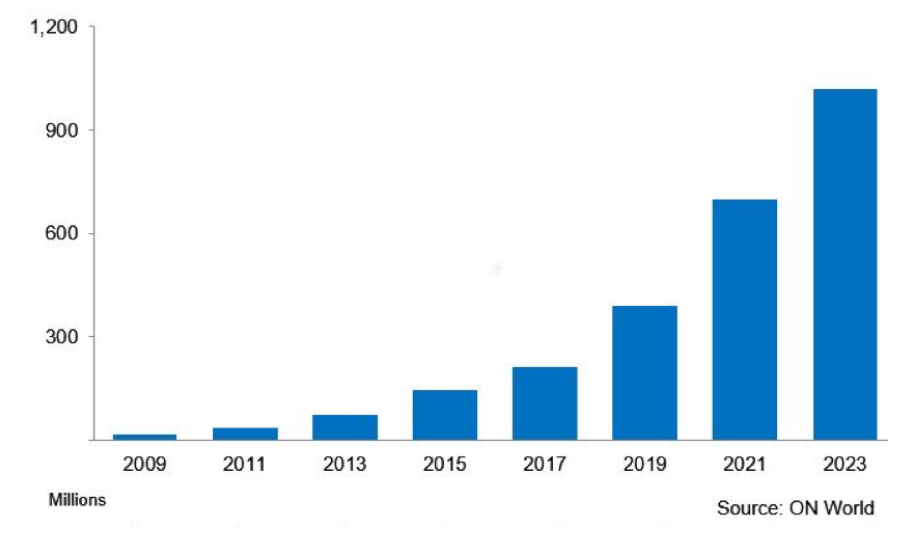
\includegraphics[width=1.0\textwidth]{sets}
\end{figure}

Zigbee chipsets are predicted to hit 1 billion shipments by 2023 (with 4.5 billion mesh devices total worldwide, most of which use Zigbee), illustrating its dominance as the most widely-used networking stack for IEEE 802.15.4 specifications. Its ease of integration with other technology stacks and hardware has seen proprietary smart home hubs such as Amazon’s Echo Plus double up as a Zigbee hub, in spite of the growth and competition from Wi-Fi and Bluetooth Low Energy (BTLE). In fact, the extremely low cost of chipsets means that developers are able to choose Zigbee/BTLE combination chips that only marginally add to the costs of manufacturing. 

Zigbee also has seen heavy adoption outside of smart home systems---commercial buildings, manufacturing and industry, municipalities, grid-based operations, and intermodal transportation systems include Zigbee as part of their technology stack (“Zigbee Leads the Wireless Mesh Sensor Network Market,” 2018). Support for medical/health devices are expected as the Zigbee Alliance looks to implement ISO/IEEE 11073 specifications into the technology stack.

The three main offerings of Zigbee are Zigbee IP, Zigbee RF4CE, and Zigbee PRO, with the lattermost being the protocol that this paper will focus on (“Network Specifications,” 2014):
\begin{itemize}
\item Zigbee IP forms the backbone of the Zigbee standard, which adds network and security layers on to the IEEE 802.15.4 standard, along with interoperability on the application layer through the Zigbee Cluster Library. It supports standard protocols such as IPv6, 6LoWPAN, TCP, TLS, UDP, and end-to-end security with TLS1.2, support for PKI, and layer 2 AES-128-CCM encryption. 
\item Zigbee RF4CE, or Radio Frequency for Consumer Electronics, offers a simple two-way, device-to-device control communication that does not require the full-featured mesh networking capabilities of Zigbee IP. 
\item Zigbee PRO is a more fully-fleshed out specification for full mesh networking capable of supporting hundreds to thousands of devices on a single network, including self-powered/energy-harvesting devices. Most developers colloquially consider non-PRO Zigbee to be a legacy, with Zigbee PRO being the standard moving forward.
\end{itemize}

\subsection{The Zigbee PRO Protocol}

The application layer gives the developer easy to use access to the data communicated over the network layer below. While the application itself is the element that will vary the most between different IoT devices, the communication needs of devices that report data and are fairly similar and limited to sending and receiving commands and data. The lack of homogeneity is instead driven by the unique physical constraints on IoT devices. Some devices, like a refrigerator that can send you a live feed of its contents, are plugged into the wall and do not need to limit their power consumption. Others, like a small sensor that checks whether a door is closed, must conserve limited battery resources as carefully as possible to avoid irritating the owner of the device. The application layer must be configured differently for each of these cases.

The network layer bridges the divide between the application layer and the physical signals received and transmitted by the radio. It also includes software used to route that data to different locations by different methods: the specification allows for a hub-and-spoke model (peripheral sensors report their data to a single devices that sends back commands), a mesh network (any device can talk to any other device), and a tree network (nodes can be simultaneously a hub to some devices and a peripheral to others). A hub-and-spoke model is the most straightforward to implement and the hub would most likely go on to report data to the internet at large to report to the company that created the devices. A mesh network is very resilient since no one point is the weakest, unlike the other two models where the hub or root of the tree are essential to operation. A tree model is good for enforcing a nuanced hierarchy of different devices, which might reflect the tasks devices are responsible for, the level of injury that a device can inflict, or the distance data can travel.

\begin{figure}[h]
	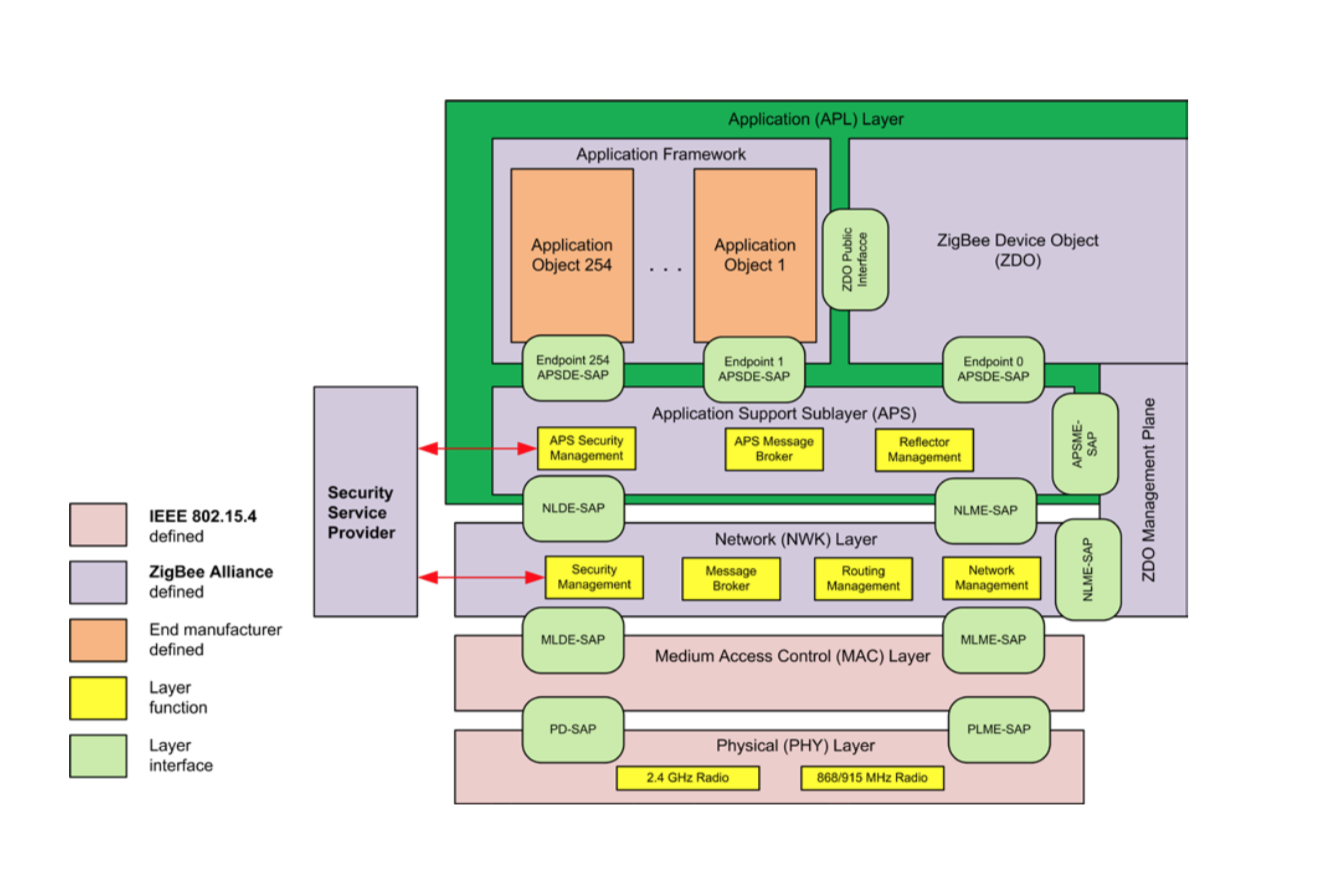
\includegraphics[width=1.0\textwidth]{top}
\end{figure}

\subsection{Threat Model: Adversaries}
Different attackers have wildly different capabilities, and therefore a suitable defense against one may be wildly insufficient (or overkill) against another. In This World Of Ours, James Mickens breaks attackers down into two basic categories: those representing governments and militaries, with effectively unlimited resources, and everyone else. (Mickens, 2014) In the case of home automation for the average, non-nation-state-actor consumer, it is reasonable to assume with some caveats that any attacker will have limited resources and all possible attacks will not be realistic. 

Mickens briefly identifies a third category of attacker: the metaphorical (or perhaps literal) angry ex-girlfriend/boyfriend, representing someone who knows the user well, may have some but not excessive technical adeptness and resources, and may have physical access. While it is important not to overlook the potential role of home automation in domestic abuse and similar situations of interpersonal violence, a New York Times report notes that the problem is usually a combination of one party having installed devices, and therefore having administrative control of them, and restraining orders and other legal measures not taking this potential means of abuse into account (Bowles). Because direct regulation of IoT is unlikely to be the best solution to this problem, this type of attack will be considered beyond the scope of this paper.

This leaves the category of attackers who are neither politically nor personally motivated. Such attackers are generally motivated by some combination of money and notoriety, and may monetize access to a stranger’s IoT device in many ways, including the following (DeSombre, 2018):
\begin{itemize}
\item Financial fraud: The attacker may directly harvest credentials and/or financial details, or they may learn other personal information which can then be used in a spearphishing attack.
\item Cryptojacking: The attacker may run cryptomining software on the victim’s device, essentially stealing computing power and electricity from them.
\item Ransomware: The attacker may implant malware than encrypts information and extorts the victim for it.
\item Botnet recruitment: The attacker may use the device to spread malware, send spam emails, participate in DDoS attacks, and so on. Aside from stolen computational resources, no money is directly taken from the victim in this case; hackers may instead charge others for the botnet’s services.
\end{itemize}

\subsection{Zigbee-Specific Vulnerability Analysis}
This section briefly evaluates how the concepts discussed in the threat model relate specifically to the Zigbee protocol. Zigbee is particularly vulnerable to attacks in which the attacker is physically near the device, and older versions add new devices in a way that is insecure. Correct implementation is key to maintaining security.

\subsection{Data Security}
Zigbee encrypts data using AES-128, a very well-established algorithm. The correctness of the algorithm itself can be considered out of scope---if AES-128 is shown to be breakable, such an exploit applied to home automation devices would be the least of everyone’s problems. The aspects of data encryption that are up to Zigbee developers are (i) correct implementation, and (ii) actually encrypting everything that should be encrypted.

Zigbee 1.2 has a known period of insecurity while a new device is being added, with developers noting it as a security vs. simplicity tradeoff and arguing that it is not feasible to have consumers instead enter security codes on all devices, since some IoT devices such as light bulbs have no reasonable means of direct user I/O (Hardawar 2015). They point out that if setting up encryption is too complicated, the user will simply not do it at all, which is far worse than accepting a split-second period of vulnerability while a secret key is being broadcast in cleartext.

Tools exist to sniff traffic and capture the unencrypted key, although exploitation requires the attacker being on the network---requiring physical proximity---during the time the key is being exchanged. Such an exploit was demonstrated at the 2015 BlackHat conference (Zillner, 2015). Zigbee 3.0 patches this flaw (Zigbee: Securing the Wireless IoT, 2017).

Because Zigbee only offers an interface to the application layer, it does not play a role in determining what data is sent to the manufacturer, and so the issue of user data being sent to manufacturers against the user’s wishes is not a part of Zigbee’s threat model.

\subsection{Device Security}
As part of the network stack, Zigbee libraries are likely to process significant amounts of untrusted, outside-originating, and therefore possibly attacker-controlled data. A bug in the Zigbee implementation---that is, something like a buffer overflow or use-after-free\footnote{These are specific, common programming errors that allow an attacker to force a machine to execute the attacker’s code rather than the intended code. They happen at a lower level of abstraction than errors such as incorrect protocol implementation that cause sensitive information not to be encrypted. In large code bases, it is very difficult to ensure that no such errors are present, and tools for definitively proving their absence are difficult to apply and have not yet found their way into widespread industry use.
} allowing for control flow hijacking, not necessarily an error in the protocol itself---would allow an attacker to take over the device.

Several attacks against device security have been demonstrated. The Python library Killerbee offers a utility for crashing Zigbee devices by connecting many spoofed stations. In itself, this is a sort of DOS attack; it also has applications as a phase of a more complete compromise, since crashed devices must reconnect to the network upon rebooting and, depending on manufacturer implementation, may broadcast keys insecurely.

In another case, researchers exploited the Zigbee stack in Philips Hue Light Bulbs to spread a worm to other devices (Ronen, 2018). They were able to remotely control lights. In addition to the obvious safety hazards and the previously-discussed possibility of devices being used in botnets, cryptomining, etc., malware spread to proximal devices presents a threat to the power grid - by controlling many devices that are located close to one another, an attacker can sharply vary the draw on a portion of the grid, which may temporarily impact availability or even damage equipment.

\subsection{Policy Landscape}
Privacy breaches are mostly covered under various privacy laws in the US, and under “data protection” rules in the European Union. In both regions, the legal frameworks draw on fair information practice principles (FIPPs) that include Transparency, Individual Participation, Purpose Specification, Data Minimization, Use Limitation, Data Quality and Integrity, Security, Accountability, and Auditing (DHS, 2014). However, different agencies emphasize different subsets of these principles. For example, while the EU legislation GDPR covers all data controllers across all industries, privacy laws are mostly domain specific in the U.S. Moreover, while there is common ground in goals on how to address privacy harms, such as advocating privacy by design, enhanced data security, and access rights to check and correct data, there are differences in how to implement these goals (in terms of obtaining consent, notification of data breaches, cross-border data flows).

\subsection{Established Regulatory Concepts}
\subsubsection{Right to be Forgotten}
Right to be forgotten provides the right to the consumer to ask for erasure of all their personal data unless there is a legitimate reason for the company to keep it (i-scoop, n.d.-b). Europe has led the efforts in identifying right to be forgotten as a fundamental right which is now accepted in other major privacy rules and regulations as such (Spiegel, 2014). 

The way this right is handled in GDPR is a good example of how the policy does not specify the technical requirements to be implemented by service providers, but simply defines the right and puts the liability on data aggregators in case of a violation. In the Home IoT context, this approach can create some ambiguity for service providers as they identify and implement new methods for how they structure data, the retention periods for different types of data, etc. (zeb, 2017).

\subsubsection{Vulnerability Notification}
The push for service providers to disclose any vulnerabilities so that the public is aware and can take necessary measures to protect themselves from further damage is another policy item that is widely accepted by most stakeholders. This principle is included in some of the policy documents shown in the table above. The industry leaders are also supporting this principle; for example, disclosure requirements were recently highlighted as a key action item by Google’s Framework for Responsible Data Protection Regulation (Enright, 2018). Transparency requirement can be seen as an alternative solution to the fact that no tamper-proof technology is available and transparency is the first step for the IoT community to do a better job in identifying problems and addressing them effectively. 

\subsubsection{Data Portability}
Defined as a fundamental right of the consumer in GDPR, data portability is a new concept (i-scoop, n.d.-a). The right to data portability is consumer centric regulation that aims to foster competition among service providers with the goal that the consumer will be able to switch between services with minimal replacement costs. GDPR defines two types of data under the portability requirement: personal data and observed data, which is the data a service provider collects as observation data while the consumer uses the service. The second data category includes IoT data. Again, data portability is required as a consumer right in the instances we observed, leaving room for service providers to identify best ways to comply as long as they take on the liability to fulfill the consumers’ needs.


\end{document}
